\chapter{Diskussion der Ergebnisse}
Die Verlustfunktion wird über $100$ Epochen bestimmt und für Trainings- und Validierungsdatensatz 
in Abbildung \ref{fig:history} dargestellt, wobei eine Batch-Size von $64$ verwendet wird. Nach ca.
$40$ Epochen bleibt der Validierungsverlust nahezu konstant, sodass weiteres Trainieren zu einer 
Überanpassung führen würde. Aus Abbildung \ref{fig:likelihood} ist ersichtlich, dass das Netz 
für den Trainingsdatensatz nur leicht bessere Vorhersagen trifft, sodass eine Überanpassung 
ausgeschlossen werden kann. Zusätzlich ist zu erkennen, dass die Verteilungen breit verteilt
sind, was die hohe \textit{cross-entropy} von $0.32$ erklärt. Es ergibt sich eine Genauigkeit 
von $0.9$ für Real News und $0.86$ für Fake News. Die in Abbildung \ref{fig:cnfsn__mtx}
dargestellte Confusion-Matrix deutet auf eine gute Performance des DNN auf dem Testdatensatz hin,
da vorallem die Hauptdiagonale ausgeprägt ist. Der hohe \textit{AUC} (area under curve)-Wert 
von $0.94$ der \textit{ROC} (receiver operating characteristic)-Kurve (Abbildung \ref{fig:roc})
deutet ebenfalls daraufhin, dass das DNN eine gute Performance hat.
\begin{figure}
    \centering
    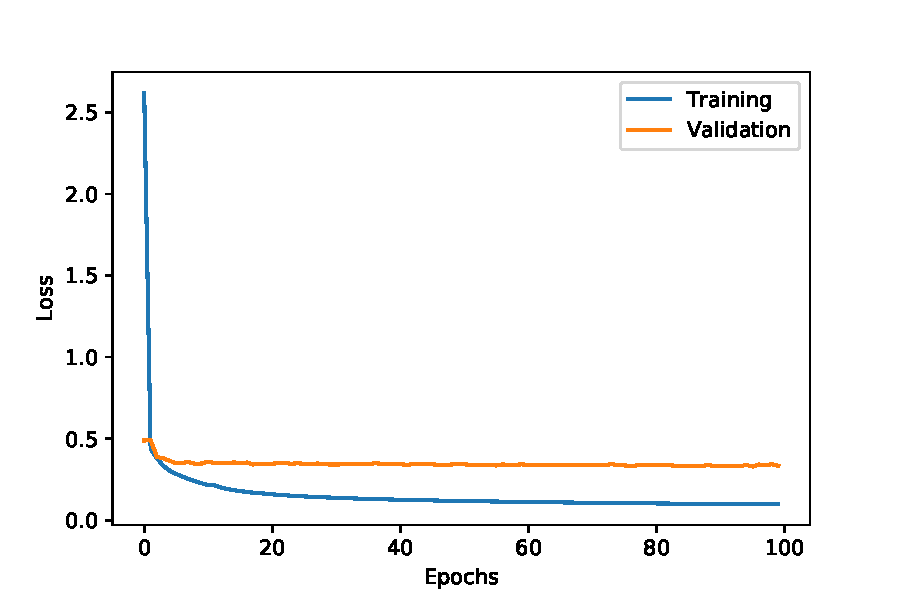
\includegraphics[width=0.8\textwidth]{pictures/history_bow_best.pdf}
    \caption{Es ist die Verlustfunktion, also \textit{cross-entropy} für Trainings- und 
    Validierungsdatensatz dargestellt. Es ist erkennbar, dass die jeweils als Real News 
    oder Fake News klassifizierten Texte, ähnliche Verteilungen besitzen.}
    \label{fig:history}
\end{figure}

\begin{figure}
    \centering
    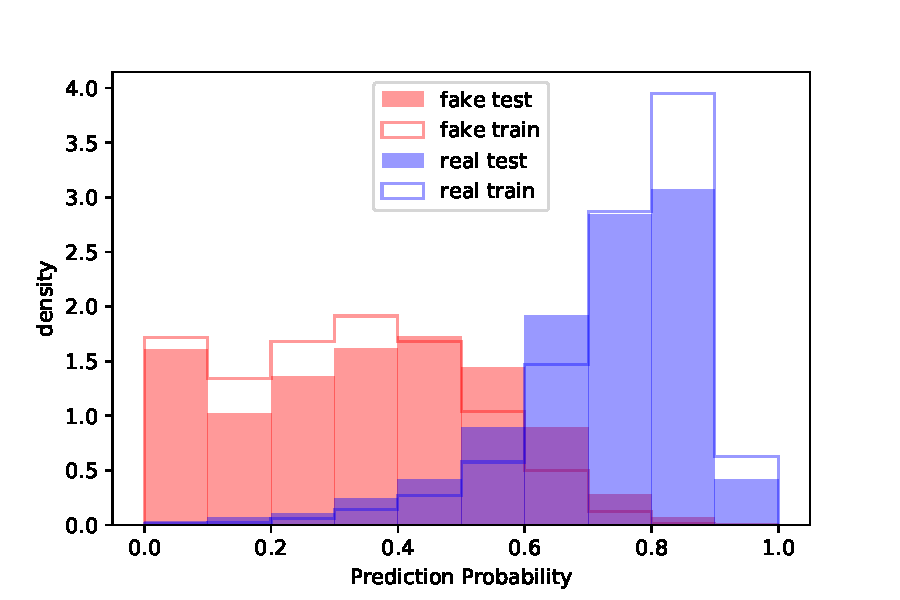
\includegraphics[width=0.8\textwidth]{pictures/prob_bow_best_nn.pdf}
    \caption{In dieser Abbildung ist die Likelihood für die verschiedenen Klassen für Trainingsdatensatz 
    und Testdatensatz dargestellt.}
    \label{fig:likelihood}
\end{figure}

\begin{figure}
    \centering
    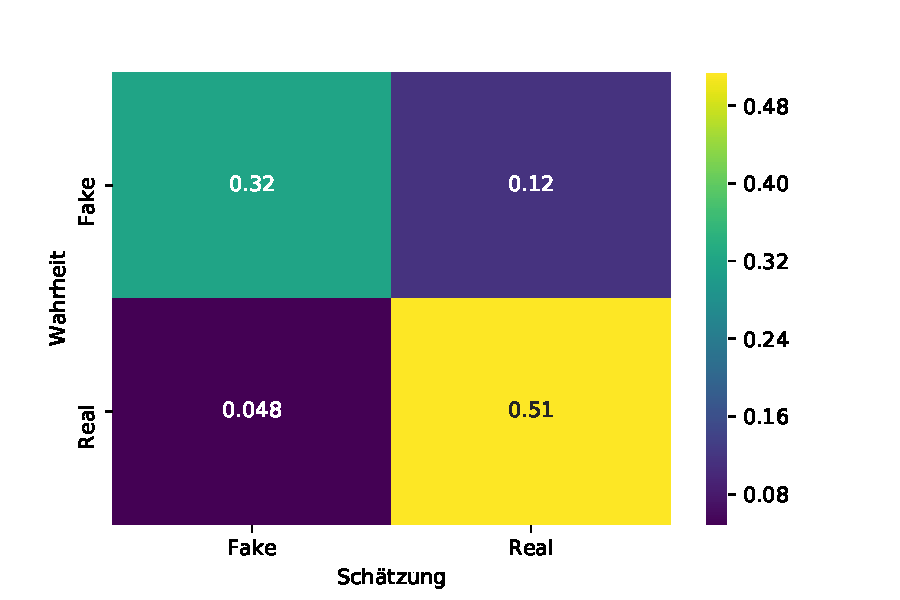
\includegraphics[width=0.8\textwidth]{pictures/cnfsn_mtx_bow_best_nn.pdf}
    \caption{Es ist die Confusion-Matrix des Testdatensatzes dargestellt. Es ist 
    zu erkennen, dass vorallem die Hauptdiagonale ausgeprägt ist, was für eine 
    gute Performance des DNN spricht.}
    \label{fig:cnfsn__mtx}
\end{figure}

Zur Interpretation der Vorhersagen des Netzes, werden die Beträge der Gewichte der ersten versteckten Lage,
die zu einem Wort gehören, aufsummiert. Unter der Annahme, dass ein hohes Gewicht einen 
hohen Einfluss auf die Vorhersage des Netzes hat, können die Wörter bestimmt werden,
die das Netz vorallem berücksichtigt. Die relativen Häufigkeiten der so bestimmten wichtigsten 
Wörter werden in einer Confusion-Matrix in Abbildung \ref{fig:cnfn_hist} dargestellt. An dieser 
Abbildung ist zu erkennen, dass die jeweils falsch klassifizierten Texte ähnliche Histogramme haben,
wie die richtig klassifizierten Texte, sodass es zu einer Verwechslung kommt. 

\begin{figure}
    \centering
    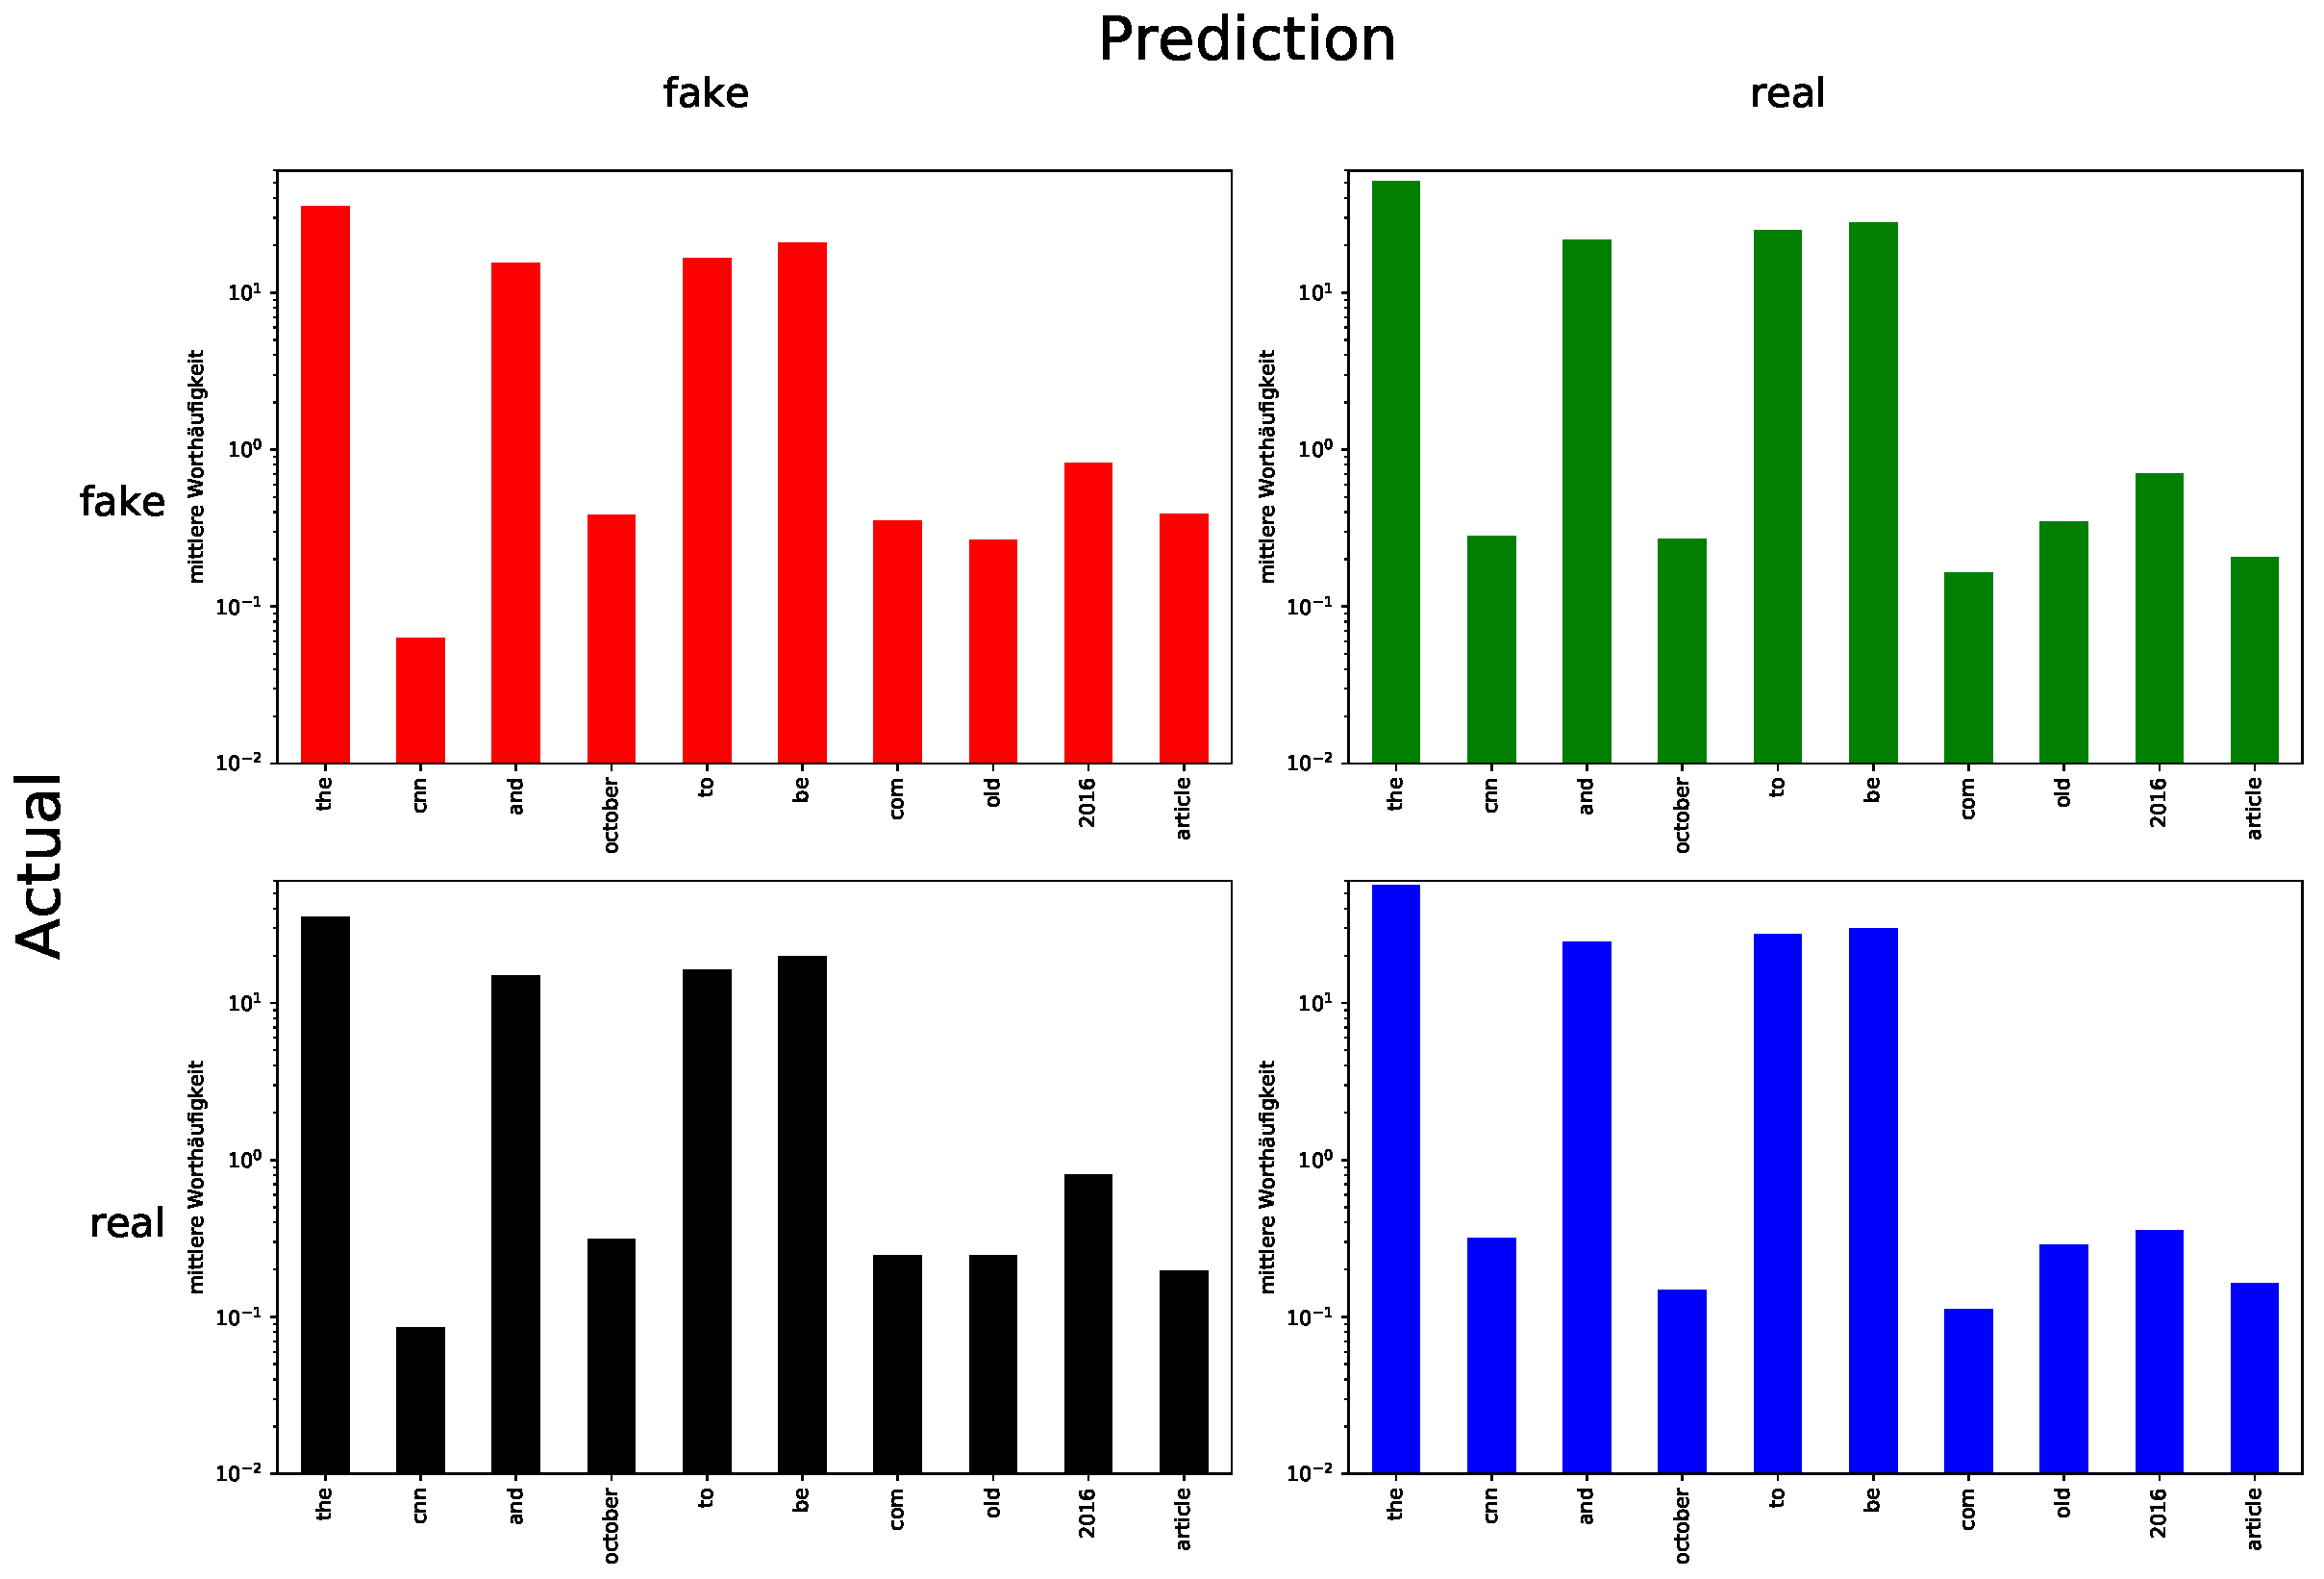
\includegraphics[width=0.8\textwidth]{pictures/cnfn_hist.pdf}
    \caption{Confusion Matrix mit relativer Häufigkeit der Wörter, die 
    im DNN stark gewichtet werden.}
    \label{fig:cnfn_hist}
\end{figure}

Beispielsweise ist das Wort \enquote{the} in den als Fake News klassifizierten Texten häufiger, als in den als 
Real News klassifizierten Texten. Es lässt sich daher vermuten, da es sich bei diesem Wort um 
ein Stoppwort handelt, sich daraus die ursprüngliche Textlänge abschätzen lässt, die im Mittel
für Real News länger ist, als für Fake News. Wichtig ist auch die Top-Level-Domain \enquote{com},
welche in den Fake News häufiger vorkommt. Dies liegt vermutlich daran, dass in den Fake News 
häufiger URL-Verlinkungen auftauchen, als in den Real News. Im Gegensatz dazu wird in Real News 
die Zeitung \enquote{CNN} häufiger erwähnt, da in diesen häufiger andere journalistische 
Zeitungen zitiert werden. Die Wichtigkeit von zeitlichen Angaben, wie \enquote{2016} und \enquote{october},
die in dem Zeitraum liegen, aus welchem die Daten stammen, lässt vermuten, dass das trainierte 
Netz sich nur für Vorhersagen aus diesem Zeitraum eignet.\\
Zum Schluss geht es um die Frage, ob die aufwendige Struktur eines DNN gerechtfertigt ist, oder 
ob es nicht möglich ist mit einem einfacheren Lösungsansatz ähnliche Ergebnisse zu erzielen. Es 
wird als Alternativmethode ein Random Forest verwendet, da dieser für Klassifizierungsaufgaben 
geeignet ist. Es wird der \textit{RandomForestClassifier} von \textsc{scikit-learn} verwendet.
Als Eingabedaten erhält dieser ebenfalls, die Bag-of-words Vektoren, besteht 
aus $100$ Entscheidungsbäumen mit maximaler Tiefe $10$ und als Einteilungskriterium die Entropie.\\
Obwohl die Hyperparameter des Random Forest nicht optimiert wurden, ergeben sich ähnliche 
Vorhersagegenauigkeiten, wie beim DNN. Die Vorhersagegenauigkeit für Real News beträgt 
$0.81$, ist also schlechter als die Vorhersagegenauikeit des DNN. Für Fake 
News ist die Genauigkeit mit $0.87$ sogar besser. Dies spiegelt sich auch in der 
\text{ROC}-Kurve (Abbildung \ref{fig:roc}) wider, die für sehr niedrigere Werte besser ist,
als die des DNN und schlechter für größere Werte. Der \textit{AUC}-Wert ist mit 
$0.92$ kleiner, als der des DNN.\\
\begin{figure}
    \centering
    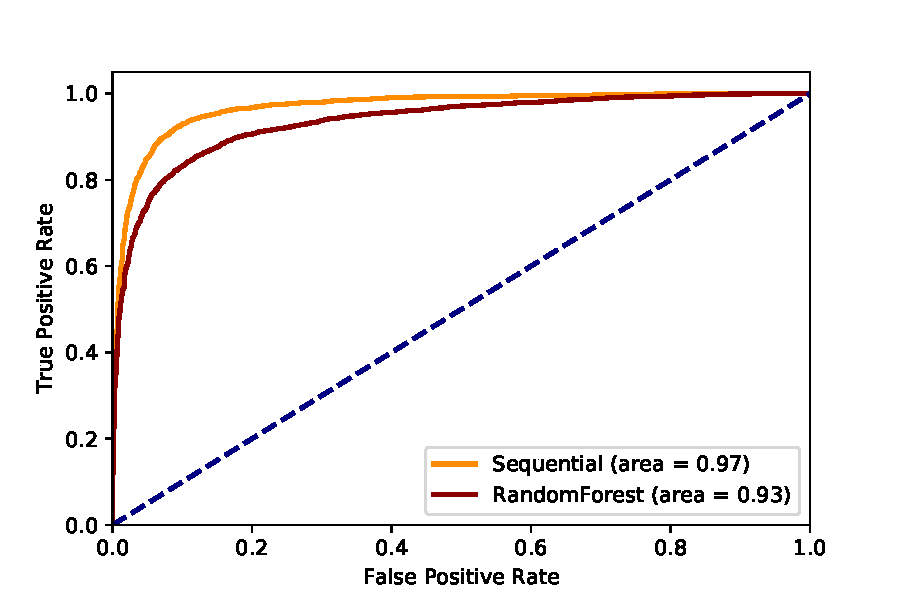
\includegraphics[width=0.8\textwidth]{pictures/roc_comparison.pdf}
    \caption{Hier ist die \text{ROC}-Kurve für das DNN und den Random Forest dargestellt.
    Beide Kurven haben einen hohen \textit{AUC}-Wert und eine nahezu rechteckige Form,
    was für eine gute Performance spricht.}
    \label{fig:roc}
\end{figure}


